\documentclass[aspectratio=169]{beamer}

\usepackage{amsmath,amssymb}
\usepackage{booktabs}
\usepackage{tabularx}
\usepackage[table,svgnames]{xcolor}
\usepackage{tikz}
\usetikzlibrary{arrows.meta,backgrounds,calc,positioning,shapes.multipart,fit}
\usepackage[main=english]{babel}
\usepackage{ragged2e}

\definecolor{fortranPurple}{HTML}{503874}
\definecolor{fortranPurpleMid}{HTML}{7E5AA6}
\definecolor{rakaliOrange}{HTML}{D9542B}

\usetheme[
  accent=fortranPurple,
  progressbar=foot,
  sectionpage=progressbar,
  numbering=fraction,
  numberrail=section,
  block=fill,
  notes=hide,
  closing=contact
]{cookie}

% Preamble (once):
%   \usepackage[table,svgnames]{xcolor}
%   \usepackage{booktabs}
%   \usepackage{tabularx}
\definecolor{cDone}{HTML}{8FD9A8}
\definecolor{cWip} {HTML}{F4C95D}
\definecolor{cTodo}{HTML}{E8918C}
\newcommand{\yes}[1]{\cellcolor{cDone}#1}
\newcommand{\prt}[1]{\cellcolor{cWip}#1}
\newcommand{\nope}[1]{\cellcolor{cTodo}#1}



\title[Fortran is cool]{Fortran is cool}
\subtitle{Don't let your friends convince you otherwise}
\author[Jorge Luis G\'alvez Vallejo \textperiodcentered\ NCI]{Jorge Luis G\'alvez Vallejo \textnormal{(NCI)}}
\cookieemail{jorge.galvezvallejo@anu.edu.au}
\institute{NCI}
\cookieuni{Australian National University}
\cookielocation{Canberra, Australia}
\date{\today}
\cookietagline{Modern Fortran, portability, and the RSE-shaped hole in scientific computing}

\titlegraphic{%
  \begin{tabular}{@{}c@{}}
    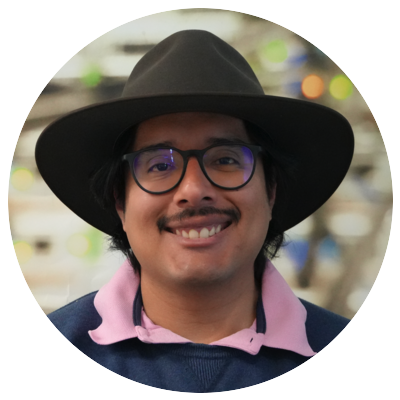
\includegraphics[height=1.6cm]{assets/jorge_c.png}\\[.7em]
    
\includegraphics[height=1.0cm]{assets/nci.png}
  \end{tabular}%
}

\cookieclosingtitle{Thank you}
\cookieclosingtext{Fortran doesn't need rewriting. It needs engineering.}
\cookieclosingqr{https://github.com/JorgeG94/pic}
\cookieclosingqrlabel{github.com/JorgeG94/pic}

\begin{document}

\maketitle

% =====================================================================
\section{The reputation}

\begin{frame}[fragile]{Your friends are half right}
  \begin{columns}[T,onlytextwidth]
    \column{.49\textwidth}
      \begin{cookiecode}[title=Fortran 77]{Fortran}
      SUBROUTINE AXPY(N,A,X,Y)
      COMMON /BLK/ SCRATCH(1000)
      DIMENSION X(1),Y(1)
      DO 10 I = 1, N
         Y(I) = A*X(I) + Y(I)
 10   CONTINUE
      RETURN
      END
      \end{cookiecode}
    \column{.49\textwidth}
      \begin{cookiecode}[title=Modern Fortran]{Fortran}
pure subroutine axpy(a, x, y)
  real, intent(in)    :: a, x(:)
  real, intent(inout) :: y(:)
  y = a*x + y
end subroutine
      \end{cookiecode}
  \end{columns}
\end{frame}


\begin{frame}{Why the debt exists}
  \begin{columns}[T,onlytextwidth]
    \column{.55\textwidth}
      \begin{itemize}
        \item These codebases were written by \textbf{scientists}, not software engineers
        \item This is a feature, not a bug
        \item Climate, weather, quantum chemistry, and CFD still run on this code. It is \textbf{not going away}
      \end{itemize}
    \column{.42\textwidth}
      \begin{block}{So}
        Not a lost cause. 
      \end{block}
  \end{columns}
  \vfill
  {\footnotesize\itshape This is the RSE-shaped hole in the talk. I will come back to it.}
\end{frame}

% =====================================================================
\section{The language}

\begin{frame}{Modern Fortran, in one slide}
  \begin{columns}[T,onlytextwidth]
    \column{.48\textwidth}
      \begin{itemize}
        \item Object orientation \cookiebadge{F2003}
        \item (Almost) safe dynamic memory --- \texttt{allocatable}, \texttt{move\_alloc}
        \item Arrays as first-class citizens --- slicing, \texttt{elemental}, reductions
      \end{itemize}
    \column{.48\textwidth}
      \begin{itemize}
        \item Native parallelism \cookiebadge{F2008}
          \begin{itemize}
            \item \texttt{do concurrent} --- shared memory + GPU
            \item coarrays --- distributed memory
          \end{itemize}
      \end{itemize}
  \end{columns}
  \vfill
  \begin{exampleblock}{The point of the whole talk}
    Fortran lets a domain scientist write \textbf{fast} code without first becoming a
    \textbf{expert programmer}.
  \end{exampleblock}
  \vspace{.2em}
  {\footnotesize\itshape I use \texttt{do concurrent}. For distributed memory I use MPI because it is just better}
\end{frame}

\begin{frame}[fragile]{One loop, every device}
  \begin{columns}[T,onlytextwidth]
    \column{.52\textwidth}
      \begin{cookiecode}[title=Standard Fortran]{Fortran}
do concurrent (k=1:nk,j=1:nj,i=1:ni)
  c(i,j,k) = al*a(i,j,k) + b(i,j,k)
end do
      \end{cookiecode}
    \column{.46\textwidth}
      \begin{cookiecode}[title=The directive wall]{Fortran}
!$omp target teams loop collapse(3)
do k = 1, nk
  do j = 1, nj
    do i = 1, ni
      c(i,j,k) = alpha*a(i,j,k) + b(i,j,k)
    end do
  end do
end do
      \end{cookiecode}
  \end{columns}
  \vspace{.3em}
  
\end{frame}

\begin{frame}{\texttt{do concurrent} across compilers}{Each vendor offloads to \emph{its} GPU --- NVIDIA is the most mature, hands down}
  \centering
  \scalebox{0.86}{\input{compiler_table_body.tex}}
\end{frame}

% =====================================================================
\section{But does it really work?}

\begin{frame}{``Sure --- for easy loops''}
  \begin{columns}[T,onlytextwidth]
    \column{.53\textwidth}
      The objection writes itself. So: the hardest realistic kernel in my field.
      \begin{itemize}
        \item \textbf{Two-electron repulsion integrals} --- irregular, deeply nested,
          the kernel everyone insists must be hand-written CUDA
        \item Prior art: Alkan \emph{et al.}, del Angel --- OpenMP target inside GAMESS,
          \textbf{per-shell-quartet}
        \item \textbf{terco}: batches of \textbf{shell pairs} dispatched to the device,
          so the GPU is never starved
      \end{itemize}
    \column{.44\textwidth}
      \begin{exampleblock}{Result}
        \centering
        {\Large\textbf{3.5$\times$ faster}}\\[.35em]
        {\footnotesize a single \textbf{V100} \\ vs.\ \textbf{Q-Chem} on 104 threads (Sapphire Rapids)}
      \end{exampleblock}
  \end{columns}
  \vspace{.2em}
  {\footnotesize OpenACC is used \textbf{only} to map data host$\leftrightarrow$device --- unneeded under unified memory.
  All parallelism is \texttt{do concurrent}.}
\end{frame}

\begin{frame}{Why not compare against cuEST?}
  \begin{columns}[T,onlytextwidth]
    \column{.55\textwidth}
      \begin{alertblock}{Because it would not be fair}
        cuEST is \textbf{density-fitted only}. \texttt{terco} evaluates
        \textbf{conventional} integrals. Comparing them would flatter me and
        mislead you.
      \end{alertblock}
    \column{.42\textwidth}
      \begin{block}{Q-Chem instead}
        Commercial, well optimized, same method. A baseline that can actually
        say no.
      \end{block}
  \end{columns}
\end{frame}

\begin{frame}{Two witnesses, four vendors}
  \begin{columns}[T,onlytextwidth]
    \column{.56\textwidth}
      {\footnotesize
      \setlength{\tabcolsep}{4pt}
      \renewcommand{\arraystretch}{1.35}
      \begin{tabularx}{\textwidth}{@{}l >{\raggedright\arraybackslash}X@{}}
        \toprule
        \textbf{Code} & \textbf{What it proves} \\
        \midrule
        \textbf{terco}        & the hardest \emph{kernel} \\
        \textbf{Rakali}       & a whole \emph{application}, 100\% Fortran \\
        \textbf{metalquicha}  & a second \emph{domain} entirely \\
        \textbf{MOM6}         & 200k lines I \emph{did not write} \\
        \bottomrule
      \end{tabularx}}
    \column{.40\textwidth}
      \begin{block}{Rakali runs on}
        {\footnotesize
        \textbf{GPUs} --- NVIDIA, AMD, Intel \\[.25em]
        \textbf{CPUs} --- Apple, ARM, Intel, AMD \\[.35em]
        One source.}
      \end{block}
  \end{columns}
  \vfill
  \begin{exampleblock}{}
    \centering Climate and quantum chemistry. Different codebases, same answer. \\
    
  \end{exampleblock}
\end{frame}

\begin{frame}{Rakali: coastal hydrodynamics, 100\% Fortran}
  \begin{columns}[T,onlytextwidth]
    \column{.5\textwidth}
      \centering
      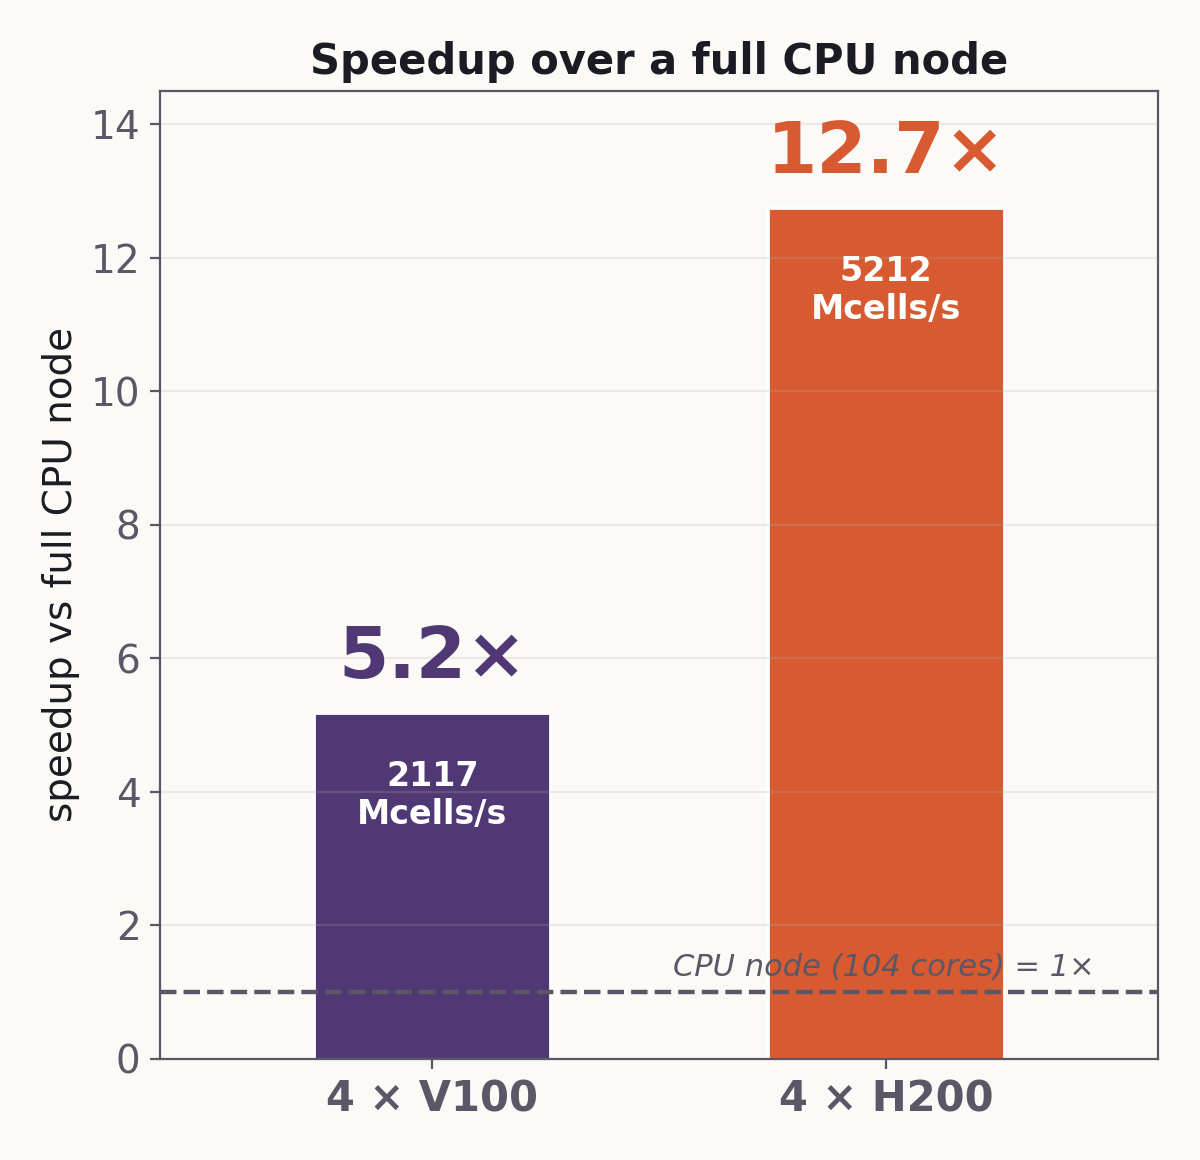
\includegraphics[width=\textwidth,height=.6\textheight,keepaspectratio]{assets/fig_speedup.png}
    \column{.48\textwidth}
      \begin{itemize}\setlength\itemsep{3pt}
        \item Coasts, rivers, floods, open ocean
        \item Lakes Entrance, Gippsland --- 30\,m grid
        \item \textbf{5.2$\times$} on 4$\times$V100, \textbf{12.7$\times$} on 4$\times$H200,
          against a full 104-core node
      \end{itemize}
      \vspace{.3em}
      \begin{block}{The honest part}
        {\footnotesize Strong scaling: V100 87\% efficient, H200 only \textbf{69\%}.
        Faster compute \textbf{exposes halo communication}. Better hardware made the
        parallel efficiency worse.}
      \end{block}
  \end{columns}
\end{frame}

% =====================================================================
\section{The ecosystem gap}

\begin{frame}{The turn: the language is portable. The ecosystem is not.}
  \begin{itemize}\setlength\itemsep{4pt}
    \item \textbf{stdlib} is genuinely good --- and in practice it builds with GNU
    \item \texttt{mpi\_f08} needs \textbf{vapaa} (Hammond) to cross compilers at all
    \item \textbf{coarrays}: elegant in F2008 --- but GCC needs OpenCoarrays, Intel ships its own
      runtime, Cray's is good, NVIDIA and AMD are nowhere
    \item Every project reimplements the same five things: sorting, logging, timers, strings, BLAS glue
  \end{itemize}
  \vfill
  \begin{alertblock}{My criterion is not ``native is good''}
    It is \textbf{portable and production-ready, or it doesn't count}.
    \texttt{do concurrent} passes. Coarrays do not --- \emph{yet}.
  \end{alertblock}
\end{frame}

\begin{frame}{A decision I made, out loud}
  \begin{cookiequote}
    I could put a coarray backend behind \texttt{pic-mpi}. I chose not to.
  \end{cookiequote}
  \vspace{.4em}
  \begin{itemize}
    \item Most coarray runtimes are \textbf{implemented on MPI} anyway --- I would be wrapping a wrapper
    \item I would owe it a \textbf{CI matrix} on compilers where coarrays barely work
    \item The abstraction would make the MPI path \emph{worse} to serve a backend I don't believe in
  \end{itemize}
  \vfill
  \begin{exampleblock}{}
    \centering That is the kind of decision Fortran codebases \\ don't get made for them often enough.
  \end{exampleblock}
\end{frame}

\begin{frame}{So I built the missing layer}
  \centering
  \begin{tikzpicture}[node distance=5mm]
    \node[cookie accent node,align=center,minimum width=9.2cm,minimum height=1.05cm] (pic)
      {\textbf{pic} --- stdlib-level routines in native Fortran \\ \footnotesize sorting \textperiodcentered\ arrays \textperiodcentered\ strings \textperiodcentered\ loggers \textperiodcentered\ timers};
    \node[cookie node,align=center,minimum width=2.9cm,minimum height=.95cm,above left=6mm and 0mm of pic.north west,anchor=south west] (blas) {\textbf{pic-blas}\\\footnotesize portable BLAS};
    \node[cookie node,align=center,minimum width=2.9cm,minimum height=.95cm,right=3mm of blas] (mpi) {\textbf{pic-mpi}\\\footnotesize distributed};
    \node[cookie node,align=center,minimum width=2.9cm,minimum height=.95cm,right=3mm of mpi] (dev) {\textbf{pic-device}\\\footnotesize device layer};
    \node[align=center,minimum width=9.2cm,minimum height=.8cm,below=6mm of pic,font=\footnotesize,draw=cookieMuted,rounded corners=3pt] (interop)
      {interop, because you are never trapped: \textbf{libfint} (libcint, ported) \textperiodcentered\ \textbf{cuEST} module interface};
    \draw[cookie arrow] (blas.south) -- (blas.south |- pic.north);
    \draw[cookie arrow] (mpi.south)  -- (mpi.south  |- pic.north);
    \draw[cookie arrow] (dev.south)  -- (dev.south  |- pic.north);
  \end{tikzpicture}
  \vspace{.6em}

  \cookiebadge{fpm} \hspace{.3em}\cookiebadge{CMake} \hspace{.3em}\cookiebadge{builds where the science builds}
\end{frame}

% =====================================================================
\section{The ask}

\begin{frame}{What RSE actually looks like in Fortran}{metalquicha --- quantum chemistry, built on the pic stack}
  \begin{columns}[T,onlytextwidth]
    \column{.5\textwidth}
      \begin{block}{Three engines, one interface}
        {\footnotesize
        \texttt{tblite} (semi-empirical, CPU) \\
        \texttt{libcint} (ab initio, CPU) \\
        \texttt{cuEST} (GPU) \\[.35em]
        All behind \texttt{qc\_method\_t}. Swap the engine --- fragmentation and screening
        are unchanged.}
      \end{block}
    \column{.48\textwidth}
      \begin{exampleblock}{The CPU path exists to be \emph{disagreed with}}
        {\footnotesize It gives the GPU path a \textbf{second, independent implementation}
        to check against --- and every method is validated against \textbf{PySCF}.}
      \end{exampleblock}
  \end{columns}
  \vspace{.5em}
  \centering
  \cookiebadge{CI} \cookiebadge{coverage} \cookiebadge{ReadTheDocs} \cookiebadge{FORD} \cookiebadge{pre-commit} \cookiebadge{contributing guide}

  \vspace{.5em}
  {\footnotesize\itshape Differential testing plus an external oracle --- exactly what scientific Fortran usually lacks.}
\end{frame}

\begin{frame}{The ask}
  \begin{cookiequote}
    Fortran does not need rewriting. It needs engineering.
  \end{cookiequote}
  \vspace{.5em}
  \begin{columns}[T,onlytextwidth]
    \column{.48\textwidth}
      \begin{itemize}
        \item CI matrices across six compilers
        \item Packaging that actually installs
        \item API design
      \end{itemize}
    \column{.48\textwidth}
      \begin{itemize}
        \item Tests, oracles, differential checks
        \item Documentation that builds
        \item Reviews
      \end{itemize}
  \end{columns}
  \vfill
  \begin{exampleblock}{}
    \centering That is RSE work. In Fortran, it is largely \textbf{unclaimed}.
  \end{exampleblock}
\end{frame}

\begin{frame}{terco means \emph{stubborn}}
  \begin{cookiequote}
    Born out of a refusal to accept that something cannot be done in plain old Fortran.
  \end{cookiequote}
  \vspace{.8em}
  \centering
  {\large So is this talk.}

  \vspace{1.2em}
  {\footnotesize
  \texttt{pic} \textperiodcentered\ \texttt{pic-blas} \textperiodcentered\ \texttt{pic-mpi} \textperiodcentered\ \texttt{pic-device} \\
  \texttt{rakali} \textperiodcentered\ \texttt{metalquicha} \textperiodcentered\ \texttt{terco} \textperiodcentered\ \texttt{libfint} \\[.4em]
  \texttt{github.com/JorgeG94} \textperiodcentered\ \texttt{fortran-lang.org}}
\end{frame}

\appendix

\begin{frame}{Backup: coarrays, if asked}
  \begin{cookiequote}
    Elegant language design --- but distributed memory is the one place where the
    ecosystem beats the language. MPI is portable today, coarrays are not, and I won't
    recommend something I wouldn't ship. If the vendors converge, I'll change my mind.
  \end{cookiequote}
\end{frame}

\end{document}
